\section{View Selection for OOD Detection}
\label{sec:propwork-mod}

%(motivation: not all views provide reasonable features, maybe we can only fuse useful views)

%The purpose of foreground-background segmentation-based views is to separate class-relevant discriminative features from potential misleading spurious features. In order to avoid spurious views, the proposed method, \textbf{M}ulti-view \textbf{O}oD \textbf{D}etection (\textbf{\sysa}), introduces a \textbf{view selector} to the fusion module in an MVCNN model . This view selector explicitly considers the discriminative features %necessary for OOD detection 
%in the foreground and background views before selecting one and using only that view for feature fusion with the original view (which is always used). The view selector is trained with a loss favoring whichever view is making more accurate predictions, based on the reasoning that a better-performing view must be extracting more meaningful semantic information with respect to ID classes. This strategy simultaneously biases the fusion module away from the misleading view and towards the view with more class-relevant discriminative features. The entire pipeline of processing multi-view data and learning the view selector is designed to be fully learnable and autonomous. %\textcolor{blue}{do we want to move the name of the method to a more strategic location instead of the first mention of it?}
Following from existing literature investigating spurious features in the context of \gls{ood} detection, the segmented view containing the \gls{id} object contains discriminative features representative of \gls{id} class objects while the remaining view likely contains primarily spurious features \cite{miyai2024locoop,neuhaus2023spurious}. In the proposed FgBg multi-view domain, the view containing discriminative or spurious features depends on the \gls{ist}. For example, an \gls{id} class of ``dog'' is clearly segmented with discriminative features in the foreground view while an \gls{id} class of ``mountain'' is segmented with discriminative features predominantly in the background (see \ref{fig:intro-mvexample}). In \gls{ood} detection, it is desired to only consider the \gls{id}-class representative discriminative features for optimal learning and separation of \gls{id} and \gls{ood} samples. Following from the previous example, if the model could automatically identify the foreground as the relevant view for the ``dog'' sample (and the background for the ``mountain'' sample), then an improved awareness of \gls{id} features would be learned and \gls{ood} data would be detected with greater accuracy.

To facilitate this idea, the proposed method, %\textbf{M}ulti-view \textbf{O}OD \textbf{D}etection (\textbf{\sysa})
\gls{sysa}, considers the novel use of a \textbf{view selector} as the fusion component in an FgBg multi-view \gls{ood} detection model. The view selector evaluates the discriminative features in the foreground and background views, selecting the superior view for fusion with the original view (which is always used, as it contains full feature information for the sample). Using a novel loss function, the view selector is trained to bias the view which has greater \gls{id} class prediction accuracy, following the assumption that increased classification performance correlates with learning of more meaningful semantic features. By leveraging this view selection mechanism, the model simultaneously rejects the view with spurious features and incorporates the additional, correlated discriminative information in the selected view.

\subsection{Proposed Method}
\label{sec:propwork-mod-propmeth}

%(proposed architecture with explanation)

%Second, each of the three views is processed using a multi-view image processing ML model. For the subsequent proposed works, the model is a multi-view convolutional NN (CNN), or MVCNN \cite{su2015multi}. An MVCNN is composed of a set of CNN feature extractors $\Phi_{V} = \{\phi_{org}, \phi_{fg}, \phi_{bg}\}$, one for each input view $v \in V$, and a fusion module $\mathcal{G}$. The CNN feature extractors are responsible for coalescing input image data into a feature vector representative of class-relevant image information, while the fusion module is responsible for regulating how much information should be included in the final model feature vector from each of its input view feature vectors. A CNN feature extractor $\phi_{v}$ takes as input its corresponding view $x_{v}$ and outputs a $p$-dimensional feature vector $z_{v} \in \mathbb{R}^{p}$, $\phi_{v}: \mathcal{X} \mapsto \mathbb{R}^{p}$. The CNN feature extractors $\Phi_{V}$ output a set of \textbf{view-specific} feature vectors \{$z_{org}$, $z_{fg}$, $z_{bg}$\} which are then passed to a fusion module $\mathcal{G}$. A fusion module $\mathcal{G}$ takes as input feature vectors from each view $v$ and outputs a combination of feature $Z_{mv}$ and prediction logits $\hat{Y}_{mv}$. %\textcolor{blue}{do we need more detail on fusion module and in general here?} 
For \gls{sysa}, the FgBg multi-view model $f_{MV}$ is implemented using a convolutional neural network (CNN) capable of processing multiple views, or \gls{mvcnn} \cite{su2015multi}, as the backbone. The multi-view feature extractors are each a CNN feature extraction backbone parameterized by $\theta$, $\phi_v = f_{\theta,v}$. Each $f_{\theta,v}$ learn view feature vectors representative of \gls{id} class information, taking as input the corresponding view $x_v$ and outputting a $d$-dimensional feature vector $z_v \in \mathbb{R}^d$, $\phi_v: \mathcal{X} \mapsto \mathbb{R}^d$. Here, $V = \{org, fg, bg\}$, and the multi-view feature extractors $\phi_{MV}$ give $Z_{MV} = \{z_{org}, z_{fg}, z_{bg}\}$. The corresponding individual classification weight matrices $W_{MV}$ and biases $b_{MV}$ give $\hat{Y}_{MV} = \{\hat{y}_{org}, \hat{y}_{fg}, \hat{y}_{bg}\}$. In \gls{sysa}, the fusion component $\mathcal{U}$ is designed with a view selector, described below, and outputs $z_{\mathcal{U}}$ and $\hat{y}_{\mathcal{U}}$.

\begin{figure}
 \centering
 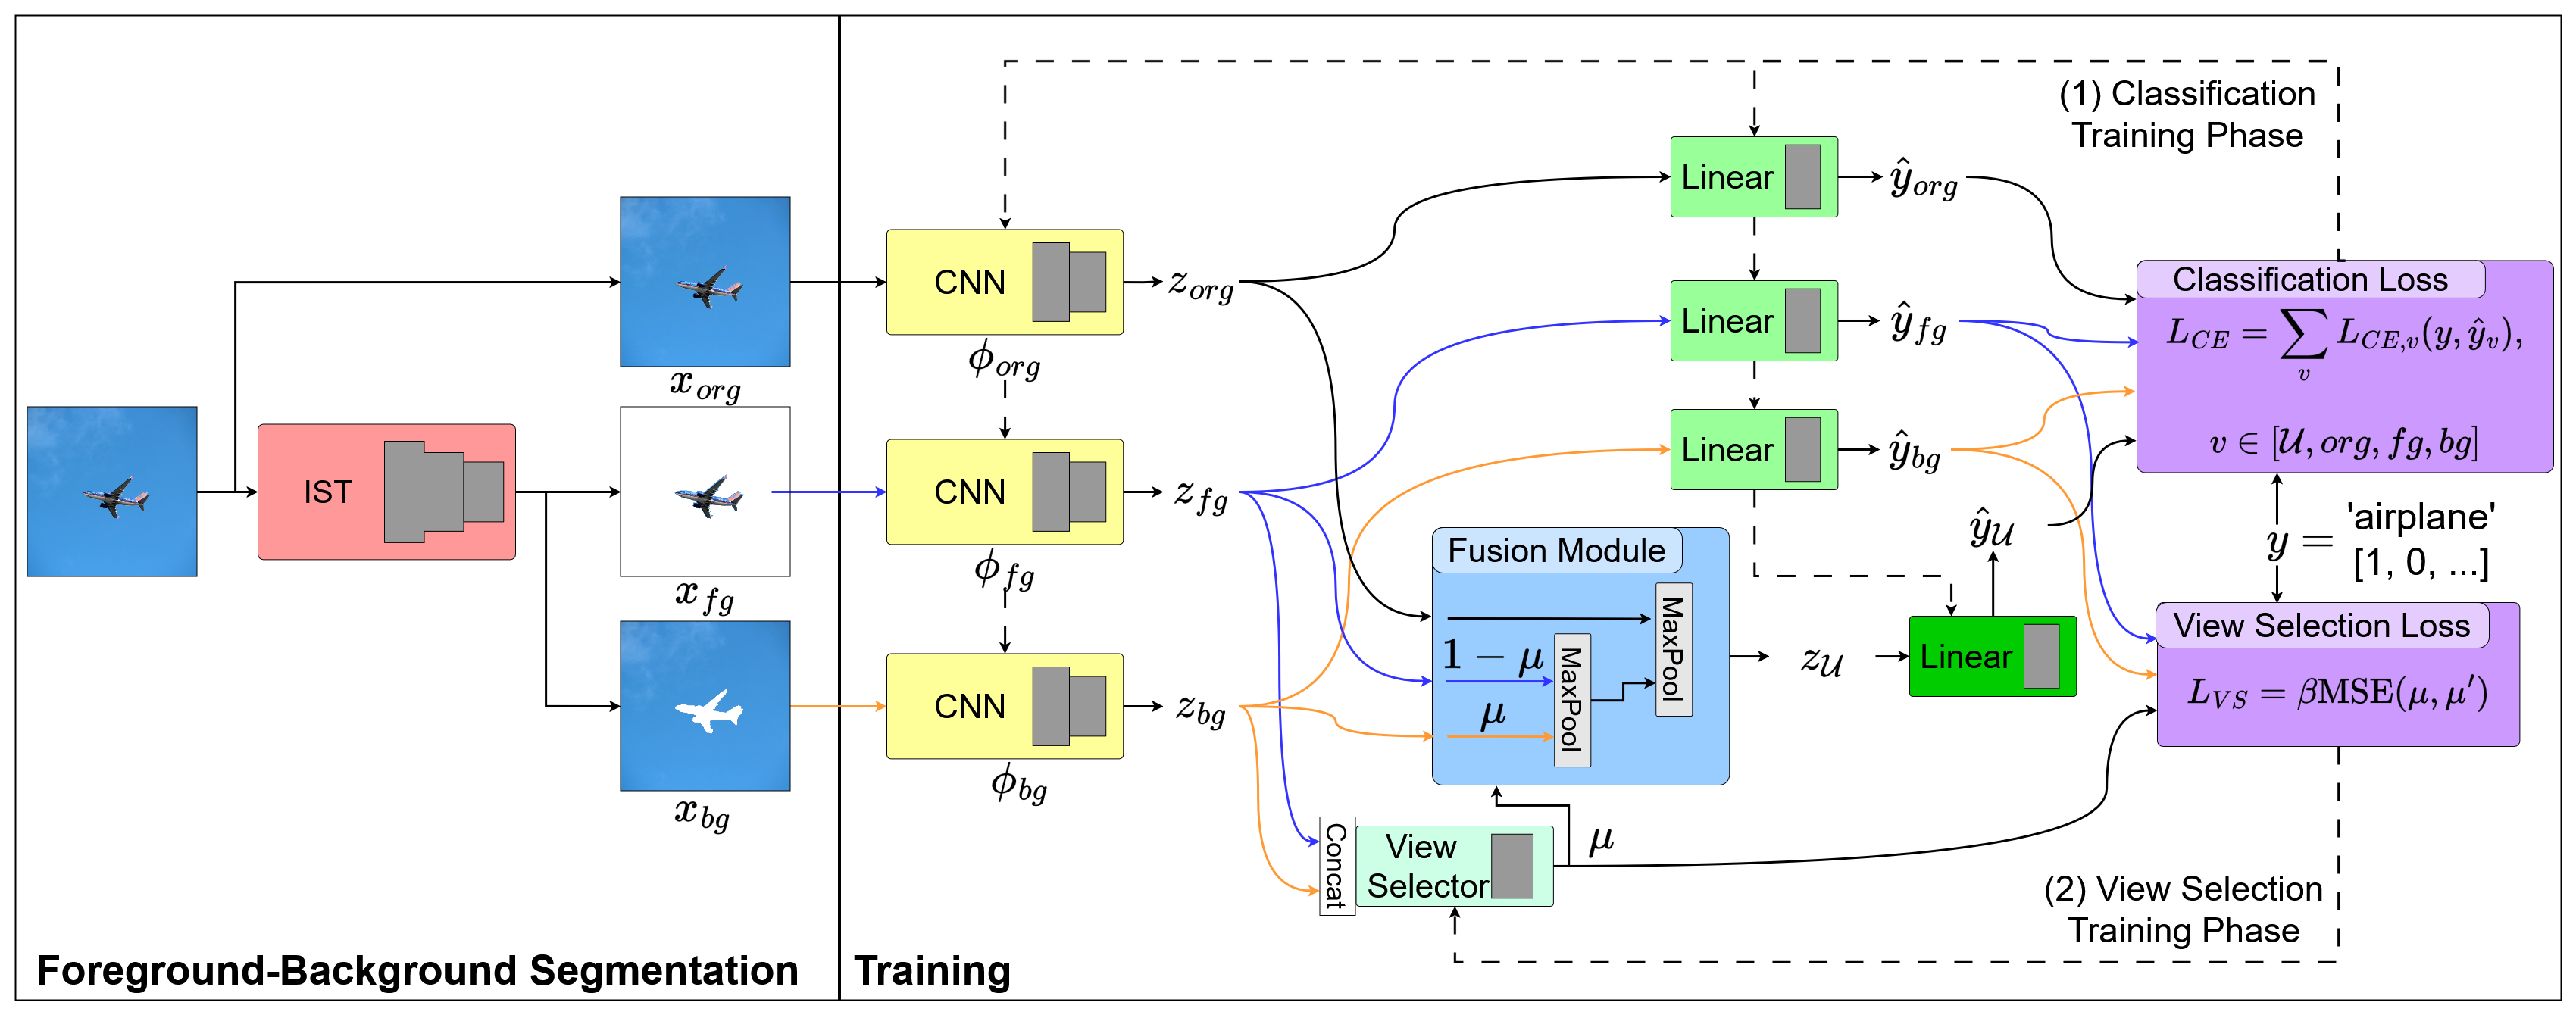
\includegraphics[width=1.\linewidth]{figures/mod_diagram}

  \caption{System diagram of the proposed \sysa. 
  Images are first foreground-background segmented using the IST before being passed to the MVCNN for processing. Note that image segmentation can be done on entire datasets as a setup step.
  Solid lines refer to forward pass, dashed lines refer to backward pass. Black lines refer to the original or fused image features. Blue lines refer to foreground image features, orange lines refer to background image features. Best viewed in color.
  }
  \label{fig:propwork-mod-diagram}
\end{figure}

%Figure \ref{fig:propwork-mod-diagram} shows the information flow of \sysa. \sysa uses an MVCNN architecture with three view inputs corresponding to the original image view (\textit{org}), the foreground view (\textit{fg}), and the background view (\textit{bg}). Each view $v \in \{org, fg, bg\}$ is passed to its corresponding view feature extractor $\phi_{v}$ resulting in three view-specific feature vectors $z_{org}$, $z_{fg}$, and $z_{bg}$. In this work, the CNN feature extractors $\Phi_{V}$ are implemented using three separate ResNet-18 \cite{he2016deep} models, although this design is modular and any model capable of taking an image as input and generating a feature vector is usable. The three view-specific feature vectors are then passed to the feature fusion module $\mathcal{G}$ which combines the three feature vectors into a fused feature vector $z_{fused} = \mathcal{G}(z_{org}, z_{fg}, z_{bg}) \in \mathbb{R}^{p}$. To enable the model to make more intelligent decisions during fusion, a \emph{view selector} is introduced that determines how much of $z_{fg}$ and $z_{bg}$ to include while producing $z_{fused}$.
The diagram in \ref{fig:propwork-mod-diagram} illustrates the high-level operations and flow of information in \gls{sysa}. An \gls{ist} segments an image into a foreground view and a background view. The \gls{mvcnn} architecture converts the input original image view (\textit{org}), foreground view (\textit{fg}), and background view (\textit{bg}) to view-specific feature vectors $Z_{MV} = \{z_{org}, z_{fg}, z_{bg}\}$. Each feature extractor $\phi_v$ in \gls{sysa} is implemented with a ResNet-18 \cite{he2016deep} model. Of note, however, is that the design of \gls{sysa} is modular. Any model capable of processing an input image and outputting a feature vector $z_v \in \mathbb{R}^d$ is compatible. The fusion component in \sysa $\mathcal{U}_{\text{\sysa}}$ uses \emph{view selection} to combine information in $Z_{MV}$ into a fused feature vector $z_{\mathcal{U}} = \mathcal{U}_{\text{\sysa}}(Z_{MV})$, $z_{\mathcal{U}} \in \mathbb{R}^d$.

%\textbf{View Selector:} The view selector is implemented via a fully connected linear layer $f$ that takes as input the concatenation of the foreground and background view-specific features $[z_{fg}; z_{bg}] \in \mathbb{R}^{2p}$. The output of the view selector is a view selection weight s
%\begin{equation}
%\begin{aligned}
%    s = \sigma(f([z_{fg}; z_{bg}]))
%\end{aligned}
%\end{equation}
%where $\sigma$ is the sigmoid function. Note that the view selector is class-agnostic.
\subsubsection{View Selector}
A critical operation in the proposed fusion component is \emph{view selection}. The view selector is implemented with a fully connected linear layer, represented by weight matrix $W_{vs}$ and bias $b_{vs}$. The foreground and background view-specific feature vectors are concatenated and used as inputs to the view selector, $[z_{fg}; z_{bg}] \in \mathbb{R}^{2d}$, where $[\cdot ; \cdot]$ represents the concatenation operation. The output is a view selection weight $\mu$
\begin{equation}
\begin{aligned}
    \mu = \sigma(W_{vs} [z_{fg}; z_{bg}] + b_{vs}),
\end{aligned}
\end{equation}
where $\sigma$ is the sigmoid function. The view selector is class-agnostic, it evaluates views based solely on the input features.

%\textbf{Fusion Module:} The view selection weight $s$ is used to weight $z_{fg}$ and $z_{bg}$ and perform max-pooling over the weighted view-specific feature vectors, resulting in a weighted foreground-background feature vector $z_{fb}$
%\begin{equation}
%\begin{aligned}
%    z_{fb} = \text{MaxPooling}_{p} \{(1-s) \cdot z_{fg}, s \cdot z_{bg}\}
%\end{aligned}
%\end{equation}
%where $\text{MaxPooling}_{p}$ is a max-pooling operation along each component in the feature dimension $p$. The fusion module $\mathcal{G}$ producing the fused feature vector $z_{fused}$ uses a final max-pooling operation over the original view-specific feature $z_{org}$ and the weighted foreground-background feature vector $z_{fb}$
%\begin{equation}
%\begin{aligned}
%    \mathcal{G}(z_{org}, z_{fg}, z_{bg}, s) = \text{MaxPooling}_{p} \{z_{org}, z_{fb}\}
%\end{aligned}
%\end{equation}
%The final fused feature vector $z_{fused}$ is the resultant output of the fusion module $\mathcal{G}$, $z_{fused} = \mathcal{G}(z_{org}, z_{fg}, z_{bg}, s)$.
\subsubsection{Fusion Component}
The fusion component $\mathcal{U}_{\text{\sysa}}$ for \gls{sysa} utilizes the view selection operation and the view features to selectively combine only the view-specific feature vectors with the most discriminative information. Specifically, the view selection weight $\mu$ weights $z_{fg}$ and $z_{bg}$ before max-pooling is performed over the weighted view-specific feature vectors. The resultant output is a weighted foreground-background feature vector $z_{fb}$
\begin{equation}
\begin{aligned}
    z_{fb} = \text{MaxPooling}_{d} \{(1-\mu) \cdot z_{fg}, \mu \cdot z_{bg}\}.
\end{aligned}
\end{equation}
$\text{MaxPooling}_{d}$ is a max-pooling operation along the feature dimension $d$. The fusion component $\mathcal{U}_{\text{\sysa}}$ outputs a fused feature vector $z_{\mathcal{U}}$, using a final max-pooling operation over the original view-specific feature $z_{org}$ and $z_{fb}$
\begin{equation}
\begin{aligned}
    z_{\mathcal{U}} = \mathcal{U}_{\text{\sysa}}(z_{org}, z_{fg}, z_{bg}, \mu) = \text{MaxPooling}_{d} \{z_{org}, z_{fb}\}.
\end{aligned}
\end{equation}

%\textbf{Prediction:} Prediction logits are produced by feeding each of the generated feature vectors, i.e. $z_{fused}$, $z_{org}$, $z_{fg}$, and $z_{bg}$, to corresponding linear layers, resulting in a fused prediction logits $\hat{y}_{fused}$ and three view-specific prediction logits $\hat{y}_{org}$, $\hat{y}_{fg}$, and $\hat{y}_{bg}$. In the proposed work experiments, only the fused prediction logits is used for ID classification, as the view-specific prediction logits are learned from limited semantic information. In summary, the final outputs of the \sysa fusion module $\mathcal{G}$ are the fused and view-specific feature vectors $Z_{mv} = \{z_{fused}, z_{org}, z_{fg}, z_{bg}\}$ and the fused and view-specific prediction logits $\hat{Y}_{mv} = \{\hat{y}_{fused}, \hat{y}_{org}, \hat{y}_{fg}, \hat{y}_{bg}\}$.
\subsubsection{Prediction}
\gls{sysa} produces logits for each of the view-specific feature vectors $Z_{MV}$ and for the fused feature vector $z_{\mathcal{U}}$. Specifically, each view-specific feature vectors in $Z_{MV}$ is passed through a corresponding linear layer, parameterized by $W_{MV}$ and $b_{MV}$, resulting in view-specific logits $\hat{Y}_{MV}$. The fused feature vector $z_{\mathcal{U}}$ is passed through a fusion linear layer with weight matrix $W_{\mathcal{U}}$ and bias $b_{\mathcal{U}}$, resulting in fused logits $\hat{y}_{\mathcal{U}}$. In \gls{sysa}, only $\hat{y}_{\mathcal{U}}$ is used for \gls{id} classification. As the fused logits learn from all correlated feature knowledge across views, they contain more \gls{id} class-relevant discriminative information for prediction. In contrast, each view-specific logits learns from (and predicts based on) limited feature information.

%\textbf{Training:} \sysa is trained using two alternating losses: a cross-entropy (CE) loss $\mathcal{L}_{CE}$ and a view selection loss $\mathcal{L}_{VS}$.
%
%$\mathcal{L}_{CE}$ is the sum of all fused and individual view CE losses. Specifically, for each view $v \in \{org, fg, bg\}$, a view-specific CE loss $\mathcal{L}_{CE,v}$ is defined as
%\begin{equation}
%\begin{aligned}
%    \mathcal{L}_{CE,v}(y, \hat{y}_{v}) = - \sum_{c \in \mathcal{Y}} y_{c} \log (\hat{y}_{v,c})
%\end{aligned}
%\end{equation}
%where $\hat{y}_{v,c}$ is the logit value of $\hat{y}_{v}$ for class $c$ and $y$ is the one-hot true label vector. The fused prediction logit CE loss $\mathcal{L}_{CE,fused}$ is defined as
%\begin{equation}
%\begin{aligned}
%    \mathcal{L}_{CE,fused}(y, \hat{y}_{fused}) = - \sum_{c \in \mathcal{Y}} y_{c} \log (\hat{y}_{fused,c})
%\end{aligned}
%\end{equation}
%where $\hat{y}_{fused,c}$ is the logit value of $\hat{y}_{fused}$ for class $c$. The final CE loss $\mathcal{L}_{CE}$ is the sum of the four losses
%\begin{equation}
%\begin{aligned}
%    \mathcal{L}_{CE} = \smashoperator{\sum_{v \in \{fused, ~org, ~fg, ~bg\}}} \mathcal{L}_{CE,v} (y, \hat{y}_{v})
%\end{aligned}
%\end{equation}
\subsubsection{Training}
\gls{sysa} is trained using two losses in an alternating optimization paradigm which has been shown to be more effective for modular architectures compared to end-to-end learning \cite{shalev2017failures,glasmachers2017limits,pascal2021improved,liu2023convergence}. The first loss is a cross-entropy (CE) loss $\mathcal{L}_{CE}$ and the second loss is a view selection loss $\mathcal{L}_{vs}$.

$\mathcal{L}_{CE}$ sums the fused and view-specific classification CE losses. For each view $v \in \{org, fg, bg\}$, a view-specific CE loss $\mathcal{L}_{CE,v}$ is defined as
\begin{equation}
\begin{aligned}
    \mathcal{L}_{CE,v}(y, \hat{y}_{v}) = - \sum_{c \in \mathcal{Y}} y_{c} \log (\hat{y}_{v,c}).
\end{aligned}
\end{equation}
$\hat{y}_{v,c}$ is the value of logit $\hat{y}_{v}$ for class $c$. $y$ is the one-hot vector of true labels for the sample. The fused CE loss $\mathcal{L}_{CE,\mathcal{U}}$ is defined as
\begin{equation}
\begin{aligned}
    \mathcal{L}_{CE,\mathcal{U}}(y, \hat{y}_{\mathcal{U}}) = - \sum_{c \in \mathcal{Y}} y_{c} \log (\hat{y}_{\mathcal{U},c}).
\end{aligned}
\end{equation}
$\hat{y}_{\mathcal{U},c}$ is the value of logit $\hat{y}_{\mathcal{U}}$ for class $c$. The final loss $\mathcal{L}_{CE}$ is the total sum of fused and view-specific CE losses
\begin{equation}
\begin{aligned}
    \mathcal{L}_{CE} = \smashoperator{\sum_{v \in \{\mathcal{U}, ~org, ~fg, ~bg\}}} \mathcal{L}_{CE,v} (y, \hat{y}_{v}).
\end{aligned}
\end{equation}

%The view selection loss $\mathcal{L}_{VS}$ is designed around the idea that, given view-specific prediction logits $\hat{y}_{v}$ ($v \in \{fg, bg\}$), low classification error using $\hat{y}_{v}$ implies that the corresponding view-specific feature $z_{v}$ (and hence, the view $v$) has encoded meaningful ID class-relevant discriminative feature information. $\mathcal{L}_{VS}$ is constructed to guide view selector learning via adjustment of $s$ towards either the foreground or the background view, minimizing classification errors associated with each view and thus improving fused features for OOD detection. This is accomplished entirely without external supervision on the value $s$. $\mathcal{L}_{VS}$ is defined as
%\begin{equation}
%\begin{aligned}
%    E_{fg} = \text{RMSE}(\hat{y}_{fg}, y) \\
%    E_{bg} = \text{RMSE}(\hat{y}_{bg}, y) \\
%    s' = \sigma(\psi (\tanh(E_{fg}) - \tanh(E_{bg}))) \\
%    \mathcal{L}_{VS} = \beta ~\text{MSE}(s, s')
%\end{aligned}
%\end{equation}
%where $E_{fg}$ and $E_{bg}$ are the Root Mean Square Errors (RMSE) corresponding to $\hat{y}_{fg}$ and $\hat{y}_{bg}$ respectively for true label vector $y$; $s'$ is the target view selection weight, set to select the view with less classification error (i.e. 0 for foreground and 1 for background) during training; and $\psi$ is a scaling factor hyperparameter and $\beta$ is a regularization hyperparameter. The view selector is influenced towards acting as a hard-gate \cite{mcculloch1943logical,fernando2017pathnet,serra2018overcoming} (i.e. exclusively selecting between the foreground and the background) via $\psi$, which serves to sharpen the sigmoid function and approximate a binary function.
The view selector component of $\mathcal{U}_{\text{\sysa}}$ learns to bias either the foreground or background view based on whichever has learned more discriminative features. A view selection loss $\mathcal{L}_{vs}$ is designed to enable this learning and operates on the classification mechanism of optimization. That is, given view-specific prediction logits $\hat{y}_{v}$ for $v \in \{fg, bg\}$, low classification error on either $\hat{y}_{v}$ represents learning of meaningful \gls{id} class-relevant discriminative feature information in the corresponding $z_{v}$. $\mathcal{L}_{vs}$ thus optimizes the view selection weight $\mu$ towards whichever view (foreground or background) with lower classification error
\begin{equation}
\begin{aligned}
    E_{fg} = \text{RMSE}(\hat{y}_{fg}, y) \\
    E_{bg} = \text{RMSE}(\hat{y}_{bg}, y) \\
    \mu' = \sigma(\psi (\tanh(E_{fg}) - \tanh(E_{bg}))) \\
    \mathcal{L}_{vs} = \delta ~\text{MSE}(\mu, \mu').
\end{aligned}
\end{equation}
$E_{fg}$ and $E_{bg}$ are Root Mean Square Errors (RMSE) on $\hat{y}_{fg}$ and $\hat{y}_{bg}$ with respect to the true label vector $y$. MSE is the Mean Square Error. \gls{sysa} uses two hyperparameters, $\psi$ which scales the difference between foreground and background error, and $\delta$ which regularizes $\mathcal{L}_{vs}$ for stability. The scaling factor $\psi$ sharpens the sigmoid function, optimizing view selection towards acting as a hard-gate and approximating a binary function \cite{mcculloch1943logical,fernando2017pathnet,serra2018overcoming}. Note that $\mu$ does not rely on any external supervision and thus does not require any user design effort.

%Using $\mathcal{L}_{CE}$ and $\mathcal{L}_{VS}$, \sysa is trained using two alternating phases. First (the \emph{classification phase}), the view selector parameters are frozen while the rest of the parameters in \sysa are trained using $\mathcal{L}_{CE}$ for some number of epochs. Then (the \emph{view-selector phase}), the view selector parameters are unfrozen while the rest of the parameters in \sysa are frozen, and the view selector is trained using $\mathcal{L}_{VS}$ for some number of epochs. This cycle repeats until both losses converge.
\gls{sysa} is trained using two alternating optimization phases, one utilizing $\mathcal{L}_{CE}$ and the other using $\mathcal{L}_{vs}$. First, in the \emph{classification phase}, view selector parameters $W_{vs}$ and $b_{vs}$ are frozen while the remaining parameters in \gls{sysa} are updated towards optimizing $\mathcal{L}_{CE}$ for a predetermined number of epochs. Then, in the \emph{view-selector phase}, $W_{vs}$ and $b_{vs}$ are unfrozen while the remaining parameters are frozen. $\mathcal{L}_{vs}$ is used to optimized the view selector parameters for another predetermined number of epochs. Both phases are repeated until all losses converge or some maximum number of epochs has passed.

%\textbf{OOD Detection:} By using three views, \sysa constructs a feature space richer in information than those of models that only use the original image view. Per previous discussion (see Section \ref{sec:intro-relwork-ood}), distance-based OOD detection methods specialize in using the feature space to identify OOD samples while avoiding the loss of information from compressing features into logits. Therefore, two state-of-the-art distance-based OOD scores, Mahalanobis Distance (MD) \cite{lee2018simple,kamoi2020mahalanobis} and k-Nearest Neighbors (KNN) \cite{sun2022out}, are analyzed for use with the proposed \sysa model. Note that both MD and KNN are \emph{post-hoc} OOD detection methods \cite{yang2022openood}, meaning that they are computed \textbf{after training has finished}. This ensures that ID classification performance of the model is preserved.
\subsubsection{OOD Detection}
A major advantage multi-view approaches have over equivalent single-view approaches is the additional correlated information within and across views. \gls{sysa} exploits this advantage by using the proposed view selector to identify and emphasize discriminative features in either the foreground or background view. Through this technique, \gls{sysa} learns a richer feature space compared to models that only use the original image. By using distance-based \gls{ood} detection methods, which specialize in leveraging the feature space to detect \gls{ood} samples without information loss (see Chapter \ref{diss_relwork}), \gls{sysa} can further exploit the multi-view advantage to achieve improved \gls{ood} detection performance. Two state-of-the-art distance-based \gls{ood} detection methods are considered: MD \cite{lee2018simple,kamoi2020mahalanobis} and KNN \cite{sun2022out}. Both MD and KNN are \emph{post-hoc} \gls{ood} detection methods \cite{yang2022openood}, i.e. they are computed \textit{after training has completed}. One of the major benefits of this is that they are generalizable across model backbones and they do not interfere with ID classification performance. For details on MD and KNN, see Chapter \ref{diss_bkgd} Section \ref{sec:bkgd-md}.

%The MD OOD score measures the distance between a sample and a Gaussian distribution. Maximum likelihood estimation is used to approximately fit class-conditional Gaussian distributions to each class in the training distribution. The empirical class means $\hat{\mu}_{c}$ and covariance matrix $\hat{\Sigma}$ are calculated from the training dataset $\mathcal{D}_{id}$ using some feature extractor $\phi$
%\begin{equation}
%\begin{aligned}
%    \hat{\mu}_{c} & = \frac{1}{N_{c}} \sum_{i:y_{i}=c} \phi(x_{i}) \\
%    \hat{\Sigma} & = \frac{1}{N} \sum_{c} \sum_{i:y_{i}=c} (\phi(x_{i}) - \hat{\mu}_{c}) (\phi(x_{i}) - \hat{\mu}_{c})^\top \\
%\end{aligned}
%\end{equation}
%where $N_{c}$ is the number of samples in class $c$. For \sysa, the feature extractor $\phi$ is replaced with the MVCNN pipeline, using the fused feature $z_{fused}$ to construct the empirical class means and covariance matrix. Given a test instance $x'$, \sysa extracts the test fused feature $z'_{fused} = \mathcal{G} (\Phi_{V}(x'_{V}), s) $ ($V = \{org, fg, bg\}$) and computes the distance between it and the nearest class-conditional Gaussian distribution, resulting in the final MD OOD score
%\begin{equation}
%\begin{aligned}
%     M_{MD}(x') = \max_{c} (-(z_{fused}' - \hat{\mu}_{c})^\top \hat{\Sigma}^{-1} (z_{fused}' - \hat{\mu}_{c})) \\
%\end{aligned}
%\end{equation}
MD in \gls{sysa} generally follows the original procedure, instead using the fused feature $z_{\mathcal{U}}$ and fused logits $\hat{y}_{\mathcal{U}}$ to calculate the empirical class means and covariance matrix. Then, given test instance $x'$, \gls{sysa} computes the test fused feature $z'_{\mathcal{U}} = \mathcal{U}_{\text{\sysa}}(Z'_{MV}, \mu')$ and the distance between $z'_{\mathcal{U}}$ and the nearest class-conditional Gaussian distribution. The resulting negative of the distance is the final \gls{sysa} MD score
\begin{equation}
\begin{aligned}
     S_{\sysa,MD}(x') = \max_{c} (-(z_{\mathcal{U}}' - \hat{\mu}_{c})^\top \hat{\Sigma}^{-1} (z_{\mathcal{U}}' - \hat{\mu}_{c})). \\
\end{aligned}
\end{equation}

%The KNN OOD score is a non-parametric distance metric that uses the $k$-th nearest neighbor distance between a test image feature vector and feature vectors from the training dataset. Previous investigations have shown that the $L_{2}$ feature norms in ID data are larger than those from OOD data \cite{tack2020csi,huang2021importance}. To account for this, the feature vectors used by \sysa in the KNN score are the normalized fused features $\zeta = \frac{z_{fused}}{\lvert \rvert z_{fused} \lvert \rvert_{2}}$. Given normalized fused feature vectors $\mathbb{Z} = \{\zeta_{i}\}^{N}$ for the training dataset $\mathcal{D}_{id}$ and a test instance $x'$, the KNN OOD score is calculated as follows. First, the normalized fused feature vector $\zeta'$ for $x'$ is generated and the Euclidean distance of $x'$ from each $x_{i} \in \mathcal{D}_{id}$ is calculated as $\lvert \rvert \zeta_{i} - \zeta' \lvert \rvert_{2}$. Second, the features in $\mathbb{Z}$ are reordered according to distance to $\zeta'$, $\mathbb{Z}' = \{\zeta_{(i)}\}^{N}$. Finally, the KNN OOD score $M_{KNN}(x')$ for $x'$ is computed as the negation of the Euclidean distance to the $k$-th ID feature
%\begin{equation}
%\begin{aligned}
%    M_{KNN}(x') = -\lvert \rvert \zeta_{(k)} - \zeta' \lvert \rvert_{2}
%\end{aligned}
%\end{equation}
%Following the conventions of OOD scores (see Section \ref{sec:intro-relwork-ood}), higher (lower) scores $M_{MD}(x')$ and $M_{KNN}(x')$ for test instance $x'$ indicate the instance is less (more) OOD.
Similarly, KNN in \gls{sysa} follows the standard KNN procedure, with $z_{\mathcal{U}}$ used to compute $\zeta_{\mathcal{U}} = \frac{z_{\mathcal{U}}}{\lvert \rvert z_{\mathcal{U}} \lvert \rvert_{2}}$ for the feature space and distance calculations. The negative of the KNN distance if the final \gls{sysa} KNN score
\begin{equation}
\begin{aligned}
    S_{\sysa,KNN}(x') =  -d_{KNN,(k)}(\zeta'_{\mathcal{U}}, \zeta_{(k)}). \\
\end{aligned}
\end{equation}

%(CIFAR-100 results: near- and far-ood)

\subsection{Experiments}
\label{sec:propwork-mod-exp}

%(VERY BASIC analysis/conclusions on results)

%Evaluation of \sysa was performed against a variety of state-of-the-art baselines and using a difficult ID dataset and several near- and far-OOD datasets \cite{yang2022openood,winkens2020contrastive}.
To evaluate \gls{sysa}, a range of near- and far-\gls{ood} datasets were considered for difficult \gls{id} domains \cite{yang2022openood,winkens2020contrastive}. A broad set of state-of-the-art baselines was used for comparison to validate the contributions of \gls{sysa}.

%\textbf{Datasets:} For training and ID testing, \textbf{CIFAR-100} \cite{krizhevsky2009learning} was used for its prevalence in the OOD detection community. It is known to be a challenging ID dataset due to its large amount of ID classes and semantic variety. For far-OOD datasets, LSUN \cite{yu2015lsun}, Textures \cite{cimpoi2014describing}, Places365 \cite{zhou2017places}, and iNaturalist \cite{van2018inaturalist} were used. For near-OOD datasets, CIFAR-10 \cite{krizhevsky2009learning} and Tiny ImageNet \cite{le2015tiny} were used.
\subsubsection{Datasets}
\textbf{CIFAR-10} and \textbf{CIFAR-100} \cite{krizhevsky2009learning}, prevalent datasets in the \gls{ood} detection literature, were used for \gls{id} training and testing \cite{yang2022openood}. The semantic similarity across samples and classes characterizes them as challenging \gls{id} datasets. Far-\gls{ood} datasets included LSUN \cite{yu2015lsun}, Textures \cite{cimpoi2014describing}, Places365 \cite{zhou2017places}, and iNaturalist \cite{van2018inaturalist}. Near-\gls{ood} datasets were Tiny ImageNet \cite{le2015tiny} and the other CIFAR dataset (i.e. CIFAR-10 near-\gls{ood} for CIFAR-100 ID, CIFAR-100 near-\gls{ood} for CIFAR-10 ID). Details for each dataset are provided below:
\begin{itemize}
\item \textbf{CIFAR-10 (C10)} \cite{krizhevsky2009learning} - A 10-class image classification dataset involving various objects, organisms, and scenes. It contains a total of 50,000 training images, 10,000 test images and 6,000 (5,000 training and 1,000 test) images per class. 
\item \textbf{CIFAR-100 (C100)} \cite{krizhevsky2009learning} - A similar image classification dataset with 100 classes. It has an identical number of training and test images with a similar train-test split (500 training and 100 testing per class). The classes and data in CIFAR-100 are distinct from those in CIFAR-10.
\item \textbf{LSUN} \cite{yu2015lsun} - A dataset containing images of objects and scenes. 10,000 images randomly sampled from its test set were used for the \gls{ood} dataset. 
\item \textbf{Textures (TXT)} \cite{cimpoi2014describing} - Images of different textures compiled into a dataset containing classes uniquely describing textures such as ``\textit{polka dotted}'' and ``\textit{bumpy}''. The entire dataset of 5,640 images was used for the \gls{ood} dataset.
\item \textbf{Places365 (Places)} \cite{zhou2017places} - A dataset containing exclusively scenes instead of the traditional objects. 10,000 images sampled randomly from the test set were used for the \gls{ood} dataset.
\item \textbf{iNaturalist (iNat)} \cite{van2018inaturalist} - An image classification dataset oriented around pictures of different species. For the \gls{ood} dataset, 10,000 images sampled from the test set were used, following previous work \cite{yang2022openood}.
\item \textbf{Tiny ImageNet (TIN)} \cite{le2015tiny} - A subset of the popular ImageNet dataset \cite{krizhevsky2012imagenet} containing 200 classes with a similar level of complexity and variety. The test set of 10,000 images was used as the \gls{ood} dataset.
\end{itemize}

A set of augmentations, including random crop, horizontal flip, and randomized rotation, was used as data transformations for each sample to improve feature learning \cite{yang2022openood,zhang2023openood,tack2020csi}. Each augmentation was generated once and applied identically to all three views of a given image. This ensures that data points maintain consistent perspectives across views when presented to the multi-view model $F_{MV}$. All images were of size 64 $\times$ 64.

%\textbf{Image Segmentation:} To perform foreground-background segmentation, the CarveKit\footnote{https://github.com/OPHoperHPO/image-background-remove-tool} open-source image background remover tool was used. CarveKit uses U2-Net \cite{qin2020u2}, a common object detection model trained on the DUTS-TR \cite{wang2017learning} dataset (which is itself a subset of the ImageNet detection dataset \cite{deng2009imagenet}), to generate the foreground and background masks. To increase efficiency, all three views for all training and testing dataset images were generated offline prior to experimentation.
\subsubsection{Image Segmentation}
A U2-Net \cite{qin2020u2} was used for foreground-background segmentation. The selected implementation of U2-Net, called CarveKit (from \href{https://github.com/OPHoperHPO/image-background-remove-tool}{https://github.com/OPHoperHPO/image-background-remove-tool}), is an off-the-shelf tool. It was chosen to demonstrate the plug-and-play nature of segmentation and foreground-background multi-view \gls{ood} detection, and is open-source software. CarveKit was trained on the DUTS-TR \cite{wang2017learning} dataset (which is a subset of the ImageNet detection dataset \cite{deng2009imagenet}). All foreground and background views for all datasets were generated prior to experimentation. %Details on other segmentation tools and performance analyses can be found in Section {\color{red}TODO}.

%\textbf{Model Architecture:} ResNet-18 \cite{he2016deep} CNN models were used as the feature extractors $\Phi_{V}$ in \sysa. The feature dimension $p$ was set to 512.
\subsubsection{Model Architecture}
The feature extractors $\phi_{MV}$ in \sysa were implemented using ResNet-18 CNN models \cite{he2016deep}. Feature dimension $d$ was set to 512.

%\textbf{Training Details:} \sysa was trained for 600 epochs with a batch size of 64, optimizer of stochastic gradient descent, learning rate of 0.1, Nesterov momentum of 0.9, and weight decay of 5e-4. Cosine annealing was used to decrease the learning rate across all epochs. $\psi$ was set to 200 and $\beta$ was set to 100. The training period for the classification phase was 5 epochs, and the training period for the view-selector phase was 1 epoch. \sysa was implemented using PyTorch, SciPy, PyTorch Lightning, and FAISS \cite{johnson2019billion}. Experiments were run on four Nvidia RTX A6000 GPUs.
\textbf{Training Details:} Detailed settings for training \gls{sysa} are:
\begin{itemize}
    \item Batch Size = 64
    \item Epochs = 600 or until convergence
    \item Optimizer = Stochastic Gradient Descent
    \item Learning Rate = 0.1
    \item Nesterov Momentum = 0.9
    \item Weight Decay = 5e-4
    \item Cosine Annealing (across all epochs)
\end{itemize}
The implementation for \gls{sysa} used PyTorch, SciPy, PyTorch Lightning, and FAISS \cite{johnson2019billion}. Computational resources utilized were four Nvidia RTX A6000 GPUs.

A grid search was performed over hyperparameters $\psi$ (50 to 300, intervals of 50) and $\delta$ (50 to 200, intervals of 50). Both were set to the optimal found value: $\psi$ was set to 200 and $\delta$ was set to 100. The classification phase training period was 5 epochs. The view-selector phase training period was 1 epoch. At test-time, the view selection weight $\mu$ was rounded to 0 or 1 to ensure no data leakage from the view which was not selected (embodying the proposed selection mechanism). Note that this enforces the effect of $\psi$ on sharpening the selection. During training, this must be used to ensure operations are differentiable during backpropagation from the view selection loss $\mathcal{L}_{vs}$.
%{\color{red}reword for experiment setup perspective}At test-time, $s$ is rounded to either 0 or 1 to ensure that only one view is chosen and prevent any data leakage from the semantically devoid view. This effectively enforces the sharpening behavior of $\psi$ which otherwise must be used during training to allow for differentiation of the view selection loss $\mathcal{L}_{VS}$ and propagation of gradients through the view selector.

%\textbf{Baselines:} The following state-of-the-art baselines were used for comparison, spanning a range of OOD detection methods: Maximum Softmax Probability (MSP) \cite{hendrycks2017baseline}, MD (with layer ensembling) \cite{lee2018simple}, KNN \cite{sun2022out}, Virtual Logit Matching (ViM) \cite{wang2022vim}, ReAct \cite{sun2021react}, Feature Normalization (FeatNorm) \cite{yu2023block}, Generalized Entropy (GEN) \cite{liu2023gen}, and Logit Normalization (LogitNorm) \cite{wei2022mitigating}. Additionally, Contrasting Shifted Instances (CSI) \cite{tack2020csi} and Class-Mixed Generation (CMG) \cite{wang2022cmg} were used for comparison on the challenging near-OOD datasets. Results for CSI and CMG were copied from the CMG paper \cite{wang2022cmg} (which has an identical experimental setup) as 1) CSI is extremely slow and a single experiment for CSI does not complete within several days, and 2) CMG uses a Variational Autoencoder \cite{kingma2014auto} model that significantly alters the training paradigm {\color{red}reword or remove}. Baseline-specific hyperparameters were selected to match those suggested or provided in each corresponding work. Note that, due to the inclusion of primarily post-hoc OOD detection methods \cite{yang2022openood} for comparison, many baselines use the same CNN model and training procedure. This explains the similar ID classification performances across methods.
\subsubsection{Baselines}
A range of state-of-the-art \gls{ood} detection methods were selected as baselines: Maximum Softmax Probability (MSP) \cite{hendrycks2017baseline}, MD \cite{lee2018simple}, KNN \cite{sun2022out}, Virtual Logit Matching (VIM) \cite{wang2022vim}, ReAct \cite{sun2021react}, Feature Normalization (FeatNorm) \cite{yu2023block}, Generalized Entropy (GEN) \cite{liu2023gen}, Logit Normalization (LogitNorm) \cite{wei2022mitigating}, Contrasting Shifted Instances (CSI) \cite{tack2020csi}, and Class-Mixed Generation (CMG) \cite{wang2022cmg}. Note that for CMG, the CMG-e variant was used as it achieves the highest performance. Results for CSI and CMG were copied from the CMG paper \cite{wang2022cmg} because it has an identical experimental setup but 1) CSI is slow to the point of being intractable (a single run of CSI takes more than a week to complete), and 2) CMG did not converge in attempted experiments. Baseline implementations used hyperparameters provided (or suggested) in the corresponding works.

%\textbf{Evaluation Metrics:} Classification accuracy is used to measure ID performance. Area under the receiver operating characteristic curve (AUROC) is used to measure OOD detection performance. All experimental results are the average of 5 random seeds. {\color{red}remove ID perf? probably - or add to later works}
\subsubsection{Evaluation Metrics}
For \gls{id} classification, Accuracy is used to measure performance. For \gls{ood} detection, Area Under the Receiver Operating Characteristic curve (AUC) is used to measure performance. All experimental results are the average of 5 random seeds.

\subsection{Results}
\label{sec:propwork-mod-results}

%(VERY BASIC analysis/conclusions on results)

%\begin{table*}
%\small
%\centering
%\caption{CIFAR-100 ID classification (\textbf{Accuracy}) and OOD detection performance (\textbf{AUROC}) comparison between \sysa and recent state-of-the-art baselines on \emph{far}-OOD datasets. All numeric values are percentages. Best results are emphasized with \textbf{boldface}.
%}
%\scalebox{1.0}{
%\begin{tabular}{|l|c|cccc|c|}
%\hline
%\multicolumn{1}{|l|}{\multirow{2}{*}{}} & ID  & \multicolumn{5}{c|}{OOD}  \\ \cline{2-7} 
%\multicolumn{1}{|l|}{} & CIFAR-100 & LSUN & Textures & Places365  & iNaturalist &  \multicolumn{1}{|c|}{Average} \\ \hline
%MSP   & 77.66$_{\pm 0.43}$   &  74.44$_{\pm 0.53}$   & 78.08$_{\pm 0.96}$   & 73.74$_{\pm 0.55}$    & \multicolumn{1}{c|}{80.24$_{\pm 0.89}$}   & 76.63  \\ 
%KNN   & 77.66$_{\pm 0.43}$   &  74.98$_{\pm 0.58}$   & 79.11$_{\pm 0.45}$   & 74.42$_{\pm 0.33}$   & \multicolumn{1}{c|}{82.48$_{\pm 0.76}$}   &  77.75 \\
%MD    & 77.66$_{\pm 0.43}$   &   68.44$_{\pm 1.56}$   & 92.92$_{\pm 0.62}$   & 69.14$_{\pm 1.38}$   & \multicolumn{1}{c|}{82.91$_{\pm 1.50}$}   & 78.35 \\
%ViM   & 77.66$_{\pm 0.43}$   &   70.04$_{\pm 1.76}$   & 83.13$_{\pm 1.20}$   & 73.15$_{\pm 0.76}$   & \multicolumn{1}{c|}{81.56$_{\pm 1.70}$}   &   76.97   \\
%ReAct & 77.66$_{\pm 0.43}$   & 72.34$_{\pm 2.54}$   & 82.41$_{\pm 2.28}$   & 76.91$_{\pm 3.12}$   & \multicolumn{1}{c|}{79.99$_{\pm 1.78}$}   &   77.91   \\ 
%FeatNorm & 77.66$_{\pm 0.43}$ & 50.51$_{\pm 2.33}$   & 74.78$_{\pm 1.98}$   & 57.25$_{\pm 1.64}$    & \multicolumn{1}{c|}{64.65$_{\pm 4.77}$}   &  61.80   \\
%GEN   & 77.66$_{\pm 0.43}$   & 73.96$_{\pm 0.63}$   & 79.04$_{\pm 1.35}$   & 73.46$_{\pm 0.89}$   & \multicolumn{1}{c|}{79.48$_{\pm 1.33}$}   &  76.49  \\ 
%LogitNorm & 75.92$_{\pm 0.55}$ &  74.56$_{\pm 0.43}$   & 75.71$_{\pm 1.98}$   & 78.54$_{\pm 0.45}$   & \multicolumn{1}{c|}{84.03$_{\pm 1.20}$}   &  77.96 \\ \hline
%\sysa-MD & \textbf{78.72}$_{\pm 0.34}$ &  \textbf{96.64}$_{\pm 2.49}$ & \textbf{95.20}$_{\pm 1.64}$ & \textbf{97.40}$_{\pm 1.27}$ & \textbf{98.53}$_{\pm 0.84}$ &  \multicolumn{1}{|c|}{\textbf{96.94}}  \\ 
%\sysa-KNN & \textbf{78.72}$_{\pm 0.34}$ &  96.51$_{\pm 2.38}$ & 94.49$_{\pm 1.91}$ & 96.86$_{\pm 1.61}$ & 98.28$_{\pm 1.23}$ &  \multicolumn{1}{|c|}{96.54} \\ \hline
%\end{tabular}
%}
%\label{tab:propwork-mod-results-cifar100-far}
%\end{table*}

%\begin{table*}
%\small
%\centering
%\caption{CIFAR-100 OOD detection performance (\textbf{AUROC}) comparison between \sysa and recent state-of-the-art baselines (incuding CSI and CMG-e) on \emph{near}-OOD datasets. All numeric values are percentages. Best results are emphasized with \textbf{boldface}.
%}
%\scalebox{1.0}{
%\begin{tabular}{|l|cc|c|}
%\hline
%\multicolumn{1}{|l|}{\multirow{2}{*}{}} & \multicolumn{3}{c|}{OOD}  \\ \cline{2-4} 
%\multicolumn{1}{|l|}{} & CIFAR-10 &  Tiny ImageNet  & \multicolumn{1}{|c|}{Average} \\ \hline
%MSP   &  78.99$_{\pm 0.20}$   & \multicolumn{1}{c|}{80.74$_{\pm 0.26}$}   & 79.87 \\
%KNN   & 77.42$_{\pm 0.36}$   & \multicolumn{1}{c|}{81.67$_{\pm 0.16}$}   &  79.55 \\
%MD    & 77.71$_{\pm 0.78}$   &  \multicolumn{1}{c|}{75.26$_{\pm 1.21}$}   &   76.49  \\
%ViM   &  71.71$_{\pm 0.94}$   & \multicolumn{1}{c|}{76.07$_{\pm 0.58}$}   &  73.89 \\
%ReAct &  78.33$_{\pm 1.36}$   & \multicolumn{1}{c|}{79.00$_{\pm 0.44}$}   & 78.67  \\
%FeatNorm & 59.81$_{\pm 1.53}$  & \multicolumn{1}{c|}{52.05$_{\pm 2.58}$}   &  55.93  \\ 
%GEN   &  80.71$_{\pm 0.47}$   & \multicolumn{1}{c|}{80.99$_{\pm 0.37}$}   & 80.85 \\
%LogitNorm & 74.68$_{\pm 0.78}$ & \multicolumn{1}{c|}{80.81$_{\pm 0.31}$}   & 77.75 \\ 
%CSI   &  78.2$_{\pm 0.2}$  &  \multicolumn{1}{c|}{79.4$_{\pm 0.2}$}     &  78.80  \\  
%CMG-e &  71.5$_{\pm 2.9}$  & \multicolumn{1}{c|}{88.2$_{\pm 2.0}$}   &  79.85 \\ \hline
%\sysa-MD & 81.66$_{\pm 6.28}$ & \textbf{91.19}$_{\pm 4.61}$ &  \multicolumn{1}{|c|}{86.43} \\ 
%\sysa-KNN & \textbf{82.68}$_{\pm 5.64}$ & 90.79$_{\pm 4.09}$ &  \multicolumn{1}{|c|}{\textbf{86.74}}  \\ \hline
%\end{tabular}
%}
%\label{tab:propwork-mod-results-cifar100-near}
%\end{table*}

\begin{table*}[h!]
\small
\centering
\caption{CIFAR-10 ID classification (\textbf{Accuracy}) and OOD detection performance (\textbf{AUC}) comparison between \sysa and recent state-of-the-art baselines. All numeric values are percentages. Best results are emphasized with \textbf{boldface}. Near-OOD datasets are marked with ``*'' and unavailable results with ``/''. ``Far'' refers to the average AUC performance across far-OOD datasets, ``Near'' refers to the average AUC performance across near-OOD datasets, and ``Avg.'' refers to the cumulative average AUC performance across all OOD datasets.
}
\vspace{0.1cm}
\scalebox{0.73}{
\begin{tabular}{|l|c|cccccc|ccc|}
\hline
\multicolumn{1}{|l|}{\multirow{2}{*}{}} & \gls{id}   & \multicolumn{9}{c|}{\gls{ood}}  \\ \cline{2-11} 
\multicolumn{1}{|l|}{}  & C10 & C100*  & LSUN   & TXT & Places & iNat & TIN* & \multicolumn{1}{|c}{Far} & Near & \multicolumn{1}{c|}{Avg.} \\ \hline
MSP   & 94.73$_{\pm 0.11}$   & 87.05$_{\pm 0.51}$   &  90.45$_{\pm 0.42}$   & 92.01$_{\pm 0.58}$   & 89.88$_{\pm 0.55}$   & 90.20$_{\pm 0.73}$   & \multicolumn{1}{c|}{87.98$_{\pm 0.34}$} & 90.63 & 87.51  & 89.59  \\  
KNN   & 94.73$_{\pm 0.11}$   & 89.55$_{\pm 0.22}$   & 92.29$_{\pm 0.15}$   & 94.24$_{\pm 0.40}$   & 91.46$_{\pm 0.25}$   & 91.73$_{\pm 0.62}$   & \multicolumn{1}{c|}{90.15$_{\pm 0.14}$}  & 92.43 & 89.85   &  91.57   \\ 
MD    & \textbf{95.37}$_{\pm 0.13}$   & 88.85$_{\pm 0.21}$   &  90.98$_{\pm 0.25}$   & 95.67$_{\pm 0.23}$   & 90.37$_{\pm 0.26}$   & 91.85$_{\pm 0.69}$   & \multicolumn{1}{c|}{89.08$_{\pm 0.18}$} & 92.22 & 88.96    &   91.13   \\  
ViM   & 94.73$_{\pm 0.11}$   & 86.39$_{\pm 1.72}$   & 89.26$_{\pm 2.05}$   & 96.05$_{\pm 1.04}$   & 88.05$_{\pm 1.96}$   & 89.96$_{\pm 1.27}$   & \multicolumn{1}{c|}{87.26$_{\pm 1.56}$}  & 90.83 & 86.82   &   89.49   \\  
React & 94.73$_{\pm 0.11}$   & 84.82$_{\pm 1.39}$   & 91.47$_{\pm 0.55}$   & 90.67$_{\pm 0.89}$   & 89.57$_{\pm 1.11}$   & 87.94$_{\pm 2.30}$   & \multicolumn{1}{c|}{86.76$_{\pm 0.98}$}  & 89.91 & 85.79   &   88.54  \\  
FeatNorm & 94.73$_{\pm 0.11}$ & 88.89$_{\pm 0.66}$  &  91.93$_{\pm 1.15}$   & 94.61$_{\pm 0.23}$   & 95.37$_{\pm 0.41}$   & 94.14$_{\pm 1.31}$   & \multicolumn{1}{c|}{90.16$_{\pm 0.81}$}  & 94.01 & 89.53  &   92.52   \\ 
GEN   & 94.73$_{\pm 0.11}$   & 87.19$_{\pm 0.58}$   &  91.35$_{\pm 0.53}$   & 92.53$_{\pm 0.79}$   & 90.82$_{\pm 0.65}$   & 90.97$_{\pm 0.90}$   & \multicolumn{1}{c|}{88.56$_{\pm 0.40}$} & 91.42 & 87.87   &   90.24  \\  
LogitNorm & 94.56$_{\pm 0.22}$ & 90.80$_{\pm 0.82}$ & 95.06$_{\pm 0.59}$   & 94.53$_{\pm 1.07}$   & 95.66$_{\pm 0.42}$   & 93.18$_{\pm 1.05}$   & \multicolumn{1}{c|}{91.80$_{\pm 0.65}$} & 94.61 & 91.30   &   93.51   \\ 
CSI  & / & 92.2$_{\pm 0.1}$     & \textbf{97.7}$_{\pm 0.4}$  & /  & /   & /   & \multicolumn{1}{c|}{\textbf{97.6}$_{\pm 0.3}$} & / & 94.90 &  /   \\  
CMG-e   & /   & 89.3$_{\pm 0.4}$   & \textbf{97.7}$_{\pm 0.9}$  & / & /  & / & \multicolumn{1}{c|}{95.2$_{\pm 2.7}$}  & / & 92.25 &    /      \\  \hline
\gls{sysa}-MD  & \textbf{95.37}$_{\pm 0.29}$ & \textbf{95.54}$_{\pm 5.39}$ & 96.02$_{\pm 2.97}$ & \textbf{98.42}$_{\pm 1.12}$ & 95.90$_{\pm 3.04}$ & \textbf{98.63}$_{\pm 0.57}$ & \multicolumn{1}{c|}{96.34$_{\pm 2.60}$}  & \textbf{97.24} & \textbf{95.94}  & \textbf{96.81}   \\ %\hline
\gls{sysa}-KNN  & \textbf{95.37}$_{\pm 0.29}$ & 95.10$_{\pm 3.73}$ & 97.37$_{\pm 1.13}$ & 97.56$_{\pm 1.17}$ & \textbf{96.48}$_{\pm 1.37}$ & 97.41$_{\pm 1.14}$ & \multicolumn{1}{c|}{96.39$_{\pm 0.91}$} & 97.21 & 95.74  &  96.72  \\ \hline
\end{tabular}
}
\label{tab:propwork-mod-results-cifar10}
\end{table*}

\begin{table*}[h!]
\small
\centering
\caption{CIFAR-100 ID classification (\textbf{Accuracy}) and OOD detection performance (\textbf{AUC}) comparison between \sysa and recent state-of-the-art baselines. 
}
\vspace{0.1cm}
\scalebox{0.73}{
\begin{tabular}{|l|c|cccccc|ccc|}
\hline
\multicolumn{1}{|l|}{\multirow{2}{*}{}} & \gls{id}  & \multicolumn{9}{c|}{\gls{ood}} \\ \cline{2-11} 
\multicolumn{1}{|l|}{}  & C100 & C10*  & LSUN   & TXT & Places & iNat & TIN* & \multicolumn{1}{|c}{Far} & Near & \multicolumn{1}{c|}{Avg.} \\ \hline
MSP   & 77.66$_{\pm 0.43}$   & 78.99$_{\pm 0.20}$   & 74.44$_{\pm 0.53}$   & 78.08$_{\pm 0.96}$   & 73.74$_{\pm 0.55}$   & 80.24$_{\pm 0.89}$   & \multicolumn{1}{c|}{80.74$_{\pm 0.26}$} & 76.63 & 79.87    & 77.71   \\
KNN   & 77.66$_{\pm 0.43}$   & 77.42$_{\pm 0.36}$   &  74.98$_{\pm 0.58}$   & 79.11$_{\pm 0.45}$   & 74.42$_{\pm 0.33}$   & 82.48$_{\pm 0.76}$   & \multicolumn{1}{c|}{81.67$_{\pm 0.16}$} & 77.75 & 79.54    &  78.35   \\ 
MD    & \textbf{78.90}$_{\pm 0.50}$   & \textbf{83.79}$_{\pm 3.10}$   &  76.71$_{\pm 0.24}$   & 88.30$_{\pm 0.66}$   & 75.08$_{\pm 0.50}$   & 84.69$_{\pm 0.60}$   & \multicolumn{1}{c|}{82.10$_{\pm 0.18}$} & 81.20 & 82.94   &   81.78   \\  
ViM   & 77.66$_{\pm 0.43}$   & 71.71$_{\pm 0.94}$   &  70.04$_{\pm 1.76}$   & 83.13$_{\pm 1.20}$   & 73.15$_{\pm 0.76}$   & 81.56$_{\pm 1.70}$   & \multicolumn{1}{c|}{76.07$_{\pm 0.58}$} & 76.97 & 73.88    &   75.94   \\  
React & 77.66$_{\pm 0.43}$   & 78.33$_{\pm 1.36}$   &  72.34$_{\pm 2.54}$   & 82.41$_{\pm 2.28}$   & 76.91$_{\pm 3.12}$   & 79.99$_{\pm 1.78}$   & \multicolumn{1}{c|}{79.00$_{\pm 0.44}$} & 77.91 & 78.66    &   78.16   \\ 
FeatNorm & 77.66$_{\pm 0.43}$ & 59.81$_{\pm 1.53}$  &  50.51$_{\pm 2.33}$   & 74.78$_{\pm 1.98}$   & 57.25$_{\pm 1.64}$   & 64.65$_{\pm 4.77}$   & \multicolumn{1}{c|}{52.05$_{\pm 2.58}$} & 61.80 & 55.93    &   59.84   \\  
GEN   & 77.66$_{\pm 0.43}$   & 80.71$_{\pm 0.47}$   &  73.96$_{\pm 0.63}$   & 79.04$_{\pm 1.35}$   & 73.46$_{\pm 0.89}$   & 79.48$_{\pm 1.33}$   & \multicolumn{1}{c|}{80.99$_{\pm 0.37}$} & 76.49 & 80.85    &  77.94   \\ 
LogitNorm & 75.92$_{\pm 0.55}$ & 74.68$_{\pm 0.78}$ & 74.56$_{\pm 0.43}$   & 75.71$_{\pm 1.98}$   & 78.54$_{\pm 0.45}$   & 84.03$_{\pm 1.20}$   & \multicolumn{1}{c|}{80.81$_{\pm 0.31}$} & 78.21 & 77.75   &   78.06 \\ 
CSI   & / & 78.2$_{\pm 0.2}$  & 80.9$_{\pm 0.5}$   & /   & /   & / & \multicolumn{1}{c|}{79.4$_{\pm 0.2}$} & /& 78.80 &    /   \\  
CMG-e & /    & 71.5$_{\pm 2.9}$  & 88.3$_{\pm 3.6}$ & /  & /   & /  & \multicolumn{1}{c|}{88.2$_{\pm 2.0}$} & / & 79.85   &  / \\ \hline
\gls{sysa}-MD & 78.72$_{\pm 0.34}$ & 81.66$_{\pm 6.28}$ & \textbf{96.64}$_{\pm 2.49}$ & \textbf{95.20}$_{\pm 1.64}$ & \textbf{97.40}$_{\pm 1.27}$ & \textbf{98.53}$_{\pm 0.84}$ & \multicolumn{1}{c|}{\textbf{91.19}$_{\pm 4.61}$} & \textbf{96.44} & \textbf{87.12}  &  \textbf{93.33}  \\ 
\gls{sysa}-KNN & 78.72$_{\pm 0.34}$ & 82.68$_{\pm 5.64}$ & 96.51$_{\pm 2.38}$ & 94.49$_{\pm 1.91}$ & 96.86$_{\pm 1.61}$ & 98.28$_{\pm 1.23}$ & \multicolumn{1}{c|}{90.79$_{\pm 4.09}$} & 95.93 & 87.08  &  92.98  \\ \hline
\end{tabular}
}
\label{tab:propwork-mod-results-cifar100}
\end{table*}


%\begin{figure}[h!]
%  \centering
%  \includegraphics[width=0.5\linewidth]{figures/selectval_error_example_B.png}
%   \caption{{\color{red}TODO}The model learns to select views which have high confidence in the correct class. Semantic information predominantly present in either the foreground or background view is automatically identified and used for fusion, classification, and OOD detection. Note that class ``\textit{dog}'' corresponds to label index 0 and class ``\textit{mountain}'' corresponds to label index 49. } 
%   \label{fig:propwork-mod-results-casestudy}
%\end{figure}

%The results are presented in Tables \ref{tab:propwork-mod-results-cifar100-far} and \ref{tab:propwork-mod-results-cifar100-near}. \sysa-MD refers to using the \sysa pipeline with MD OOD score and \sysa-KNN refers to using the \sysa pipeline with KNN OOD score. For far-OOD datasets (Table \ref{tab:propwork-mod-results-cifar100-far}), on average \sysa outperformed all previous state-of-the-art baselines, with \sysa-MD improving on the best baseline AUROC by 18.59\%. Furthermore, both \sysa-MD and \sysa-KNN outperformed all baselines in all far-OOD datasets. For near-OOD datasets (Table \ref{tab:propwork-mod-results-cifar100-near}), \sysa-MD and \sysa-KNN likewise outperformed all baselines, both on average (maximum AUROC improvement of 5.89\% in \sysa-KNN) and in each near-OOD dataset. \sysa does not negatively impact ID classification (see Table \ref{tab:propwork-mod-results-cifar100-far}), instead improving accuracy on the CIFAR-100 test set by 1.06\%. Of note is that \sysa performs well on ID classification and OOD detection across both near- and far-OOD datasets with \textbf{both MD and KNN OOD scores}. This suggests that \sysa learns robust feature spaces beneficial to both statistical distance measures (MD) and non-parametric distance metrics (KNN). The results further suggest that \sysa successfully learns ID class-relevant discriminative features. Far-OOD datasets are defined as containing features that are very different from ID discriminative features. The significant improvement in OOD detection performance across far-OOD datasets indicates \sysa learned to identify the clear spurious features in the views of far-OOD data, easily distinguishing such samples from ID samples. For near-OOD datasets, this effect is less pronounced but still evident as OOD detection in near-OOD settings requires models to use ID discriminative features to identify ID samples and reject OOD samples. 
The results, detailed in \ref{tab:propwork-mod-results-cifar10} (for CIFAR-10) and \ref{tab:propwork-mod-results-cifar100} (for CIFAR-100), demonstrate that \gls{sysa} improves \gls{ood} detection performance over single-view baselines. Note that \gls{sysa}-MD refers to using MD with \gls{sysa} and \gls{sysa}-KNN refers to using KNN with \gls{sysa}. Comparisons of average results here do not consider CSI and CMG-e as results are not available for all datasets. For far-\gls{ood} datasets, \gls{sysa} outperforms all previous state-of-the-art baselines on average in both the CIFAR-10 and CIFAR-100 experimental settings. \gls{sysa}-MD improves on the best baseline AUC by 2.63\% with CIFAR-10 and by 18.59\% with CIFAR-100. With CIFAR-10, both \gls{sysa}-MD and \gls{sysa}-KNN outperform baselines across all far-\gls{ood} datasets except LSUN, in which \gls{sysa}-KNN underperforms by only 0.33\%. With CIFAR-100, both \gls{sysa}-MD and \gls{sysa}-KNN outperform all baselines across the far-\gls{ood} datasets. For near-\gls{ood} datasets, all baselines are again outperformed on average by \gls{sysa}-MD and \gls{sysa}-KNN. With CIFAR-10, \gls{sysa}-MD improves the maximum AUC by 1.04\% on average and by 3.34\% in CIFAR-100. \gls{sysa}-KNN improves the maximum AUC by 0.84\% on average and by 2.9\% in CIFAR-100. In Tiny ImageNet, \gls{sysa} only underperforms compared to CSI by 1.21\%. With CIFAR-100, \gls{sysa}-MD improves the maximum AUC by 4.18\% on average and by 2.99\% in Tiny ImageNet. \gls{sysa}-KNN improves the maximum AUC by 4.14\% on average and by 2.59\% in Tiny ImageNet. Similar to the CIFAR-10 setting, \gls{sysa} only underperforms MD in CIFAR-10 by 1.11\%. Overall, \gls{sysa} improves over state-of-the-art baselines in \gls{ood} detection by 3.30\% for CIFAR-10 and by 11.55\% for CIFAR-100 (both with \gls{sysa}-MD, but \gls{sysa}-KNN only differs by 0.09\% and 0.35\% respectively).

Due to using post-hoc \gls{ood} detection methods, \gls{sysa} preserves \gls{id} classification performance. Crucially, \gls{sysa} achieves competitive \gls{id} classification and state-of-the-art \gls{ood} detection performance with \textbf{both MD and KNN \gls{ood} scores} across \textbf{both near- and far-\gls{ood} datasets}. As mentioned, for CIFAR-10, the difference between average AUC for \gls{sysa}-MD and \gls{sysa}-KNN is merely 0.09\%. This gap is small for CIFAR-100 too, only 0.35\%. This suggests that \gls{sysa} successfully leverages the complementary feature information in multiple views to learn feature spaces robust to both MD (statistical distance metric) and KNN (non-parametric distance metric). Furthermore, the results indicate that \gls{sysa} learns comprehensive \gls{id} class-relevant discriminative features, leading to not only high classification accuracy but improved \gls{ood} detection. This is easily visible in the performance of \gls{sysa} on far-\gls{ood} datasets, where features are significantly different from those in \gls{id} data (18.59\% improvement for \gls{sysa}-MD in CIFAR-100). The improved AUC implies that \gls{sysa} clearly identifies and detects the spurious features in far-\gls{ood} views. For near-\gls{ood} data, this improved AUC reflects a similar narrative as improving \gls{ood} detection performance in near-\gls{ood} domains requires learning of \gls{id} discriminative features.

\begin{table*}[htp!]
\small
\centering
\caption{
Ablation results for CIFAR-100 ID classification (Accuracy) and OOD detection performance (AUC) between \sysa, basic multi-view classification techniques, and different view inclusions during feature fusion. Learned view selection method outperforms all other configurations in ID accuracy and average OOD detection performance, showing a need for intelligent feature fusion.}
\vspace{0.1cm}
\scalebox{0.9}{
\begin{tabular}{|l|c|ccccccccc|}
\hline
\multirow{2}{*}{} & \gls{id}  & \multicolumn{9}{c|}{\gls{ood}}   \\ \cline{2-11} 
\multicolumn{1}{|l|}{}  & C100 & C10*  & LSUN   & TXT & Places & iNat & TIN* & \multicolumn{1}{|c}{Far} & Near & \multicolumn{1}{c|}{Avg.} \\ \hline
Org-only  & 77.63 &  79.45  &  82.01  & 73.04  & 74.82 & 76.76  & \multicolumn{1}{c|}{74.23}  & 76.66 & 76.84 &  76.72  \\ 
Fg-only   & 72.06 & 75.95  & 83.05  & 77.67  & 83.06  & 83.79  & \multicolumn{1}{c|}{80.50}  & 81.89 & 78.23 &   80.67  \\ 
Bg-only   & 20.49 & 58.18 &  90.51 & \textbf{96.21} & 91.94 & 94.96 & \multicolumn{1}{c|}{\textbf{95.82}}  & 93.41 & 77.00 &  87.94   \\ \cdashline{1-11}
Org-Fg    & 77.98 & 79.52 &  93.92  & 86.83  & 94.62  & 96.10  & \multicolumn{1}{c|}{84.52}   & 92.87 & 82.02 &   89.25 \\ 
Org-Bg    & 76.90 & \textbf{88.54}  & 90.91  & 93.75  & 86.13  & 89.97  & \multicolumn{1}{c|}{90.28}  & 90.19 & 89.37 &  89.93  \\ 
Fg-Bg & 71.76   & 86.55  &  90.35  & 95.99  & 89.12 & 91.61   & \multicolumn{1}{c|}{94.58}  & 91.77 & \textbf{90.57} &  91.37  \\ \cdashline{1-11}
Org-Fg-Bg & 77.94  & 79.13  &  83.66  & 77.45  & 77.57 & 78.59  & \multicolumn{1}{c|}{71.05}  & 79.29 & 75.09 & 77.91 \\ 
Ensemble (Mean) & 77.01 & 79.90  &  88.50  & 84.37 & 85.78  & 87.69 & \multicolumn{1}{c|}{85.50}   & 86.59 & 82.70 &   85.29 \\ 
Ensemble (Max) & 75.84  & 78.48    &  88.66    &  79.89   & 83.21    & 85.48 & \multicolumn{1}{c|}{81.26}   & 84.31 & 79.87 &  82.83 \\ 
Ensemble (Min) & 67.43   & 77.50    &  86.34    &  83.84   & 84.52    & 85.65  & \multicolumn{1}{c|}{85.11}   & 85.09 & 81.31 &  83.83  \\ \hline
\gls{sysa} & \textbf{78.72} & 81.66 &  \textbf{96.64}  & 95.20  & \textbf{97.40}  & \textbf{98.53}  & \multicolumn{1}{c|}{91.19} & \textbf{96.94} & 86.43 &   \textbf{93.33} \\ \hline
\end{tabular}
}
\label{tab:propwork-mod-results-ablations}
\end{table*}

\subsubsection{Ablation Study}
To analyze the performance contributions of each view, a set of ablation experiments were performed over all combinations of original (Org), foreground (Fg) and background (Bg) views. Single-view experiments (i.e. Org-only, Fg-only, and Bg-only) used only the respective CNN feature extraction backbone $\phi_v$ and linear prediction head $W_v, b_v$ for testing. View-combination experiments (i.e. Org-Fg, Org-Bg, Fg-Bg) were evaluated by max-pooling the corresponding two view feature vectors and adding a separate linear prediction head for the combination during training and testing. The all-view experiments used naive combinations of all views, either through max-pooling of all view features (i.e. Org-Fg-Bg) or through ensembling (i.e. Ensemble), of which mean, max, and min ensembling were considered.

The results of the study are presented in \ref{tab:propwork-mod-results-ablations}. Overall, \gls{sysa} improves both \gls{id} classification and \gls{ood} detection performance over all other combinations of views and naive fusion methods. As expected, Org-only achieves high \gls{id} classification performance, but \gls{sysa} still improves over it by 1.09\%. Surprisingly, Bg-only achieves respectable \gls{ood} detection performance, even outperforming all other ablation settings and \gls{sysa} in Textures and Tiny ImageNet. However, the lack of foreground information significantly reduces the \gls{id} classification performance (a difference of 58.23\% compared to \sysa) and fails to outperform \gls{sysa} in \gls{ood} detection on average (a difference of 5.39\%). Combining views generally improves performance, with Org-Fg, Org-Bg, and Fg-Bg all outperforming single-view experiments in overall average \gls{ood} detection. It is observed that the presence of the Bg view improves \gls{ood} detection, specifically near-\gls{ood} detection. Org-Bg and Fg-Bg significantly outperform other view combinations, with Fg-Bg achieving the highest near-\gls{ood} detection performance, 4.14\% over \gls{sysa}. However, following previous observations, the Bg view degrades \gls{id} classification, with Org-Bg decreasing accuracy by 1.08\% and Fg-Bg decreasing accuracy by 6.22\% (both with respect to Org-Fg).
\gls{sysa} also significantly improves on the baseline fusion Org-Fg-Bg which does not intelligently consider the semantic contributions of views. Furthermore, Org-Fg-Bg does not use view-specific losses in training and performs worse in \gls{id} classification accuracy, by 0.78\%, and significantly worse in \gls{ood} detection, by 15.42\% on average. This introduces a significant contributing notion regarding multi-view \gls{ood} detection: simply including more views is not necessarily sufficient to improve performance, some form of \textit{intelligent fusion of view information} is necessary.
Furthermore, this verifies the notion that training each view to extract semantically-meaningful discriminative features critically impacts model performance in handling both \gls{id} and \gls{ood} data. 

For ensembling, \gls{id} view-specific prediction logits $\hat{y}_{org}$, $\hat{y}_{fg}$, $\hat{y}_{bg}$ are converted into probabilities via softmax and then combined across views (averaged for mean, max and min for their respective methods), resulting in a final aggregate prediction probability distribution. A similar procedure is used for \gls{ood} scores, with \gls{ood} scores calculated for each view feature vector $z_{org}$, $z_{fg}$, $z_{bg}$ and combined across views, resulting in a final aggregate \gls{ood} score. It is clear that ensembling does not outperform the discriminative feature-aware view selection used in \gls{sysa} fusion. This follows multi-view classification literature: it has been shown that feature fusion significantly outperforms ensembling of prediction scores \cite{seeland2021multi}.

\gls{sysa} performs the best in \gls{id} classification, average \gls{ood} detection, and far-\gls{ood} detection, all across a range of \gls{ood} datasets. This, along with the aforementioned observations across view combinations, supports the conclusion that \emph{principled fusion} is critical to extraction and learning of discriminative features. The informed view selection fusion mechanism proposed in \gls{sysa} enables this discriminative feature learning and thus improves \gls{ood} detection. However, \gls{sysa} underperforms in near-\gls{ood} detection. It has already been observed that consideration of the Bg view improves near-\gls{ood} detection performance. It is hypothesized that this is because the background feature extraction backbone tends to reject unfamiliar, spurious features. Observations on background predictions showed a tendency towards more uniform confidence distributions for all samples with few discriminative features in the background view. If \gls{sysa} biased the foreground view over the background view during selection, it would not have access to the Bg view information for near-\gls{ood} detection, leading to decreased performance.

\begin{table}
\small
\centering
\caption{View selector performance on a curated dataset. The view selector learns to identify views with discriminative features. All numeric values are percentages except for support.
}
\vspace{0.1cm}
\scalebox{1.}{
\begin{tabular}{|l|ccc|c|}
\hline
\multicolumn{1}{|l|}{}   & \multicolumn{1}{c}{Precision}     & \multicolumn{1}{c}{Recall}        & \multicolumn{1}{c}{F-Score} & \multicolumn{1}{|c|}{Support} \\ \hline
\multicolumn{1}{|l|}{Foreground} &  \multicolumn{1}{c}{80.83}   &  \multicolumn{1}{c}{97.00}   & 88.18 & \multicolumn{1}{|c|}{100}  \\  
\multicolumn{1}{|l|}{Background} &  \multicolumn{1}{c}{96.25}   &  \multicolumn{1}{c}{77.00}   & 85.56 & \multicolumn{1}{|c|}{100}  \\  \hline
\multicolumn{1}{|l|}{Accuracy} & 87.00 & \multicolumn{2}{c}{} &  \multicolumn{1}{|c|}{200}     \\ \hline
\end{tabular}
}
\label{tab:propwork-mod-results-view_selector_performance}
\end{table}

\begin{table*}[htp!]
\small
\centering
\caption{
View selector foreground-selection frequency on CIFAR-100 testing ID and OOD datasets.}
\vspace{0.1cm}
\scalebox{1.}{
\begin{tabular}{|l|c|cccccc|}
\hline
\multirow{2}{*}{} & \gls{id} & \multicolumn{6}{c|}{\gls{ood}}  \\ \cline{2-8} 
& C-100  & C-10* & LSUN & TXT & Places & iNat & \multicolumn{1}{c|}{TIN*} \\ \hline
Frequency  & 0.961  & 0.816 & 0.799 & 0.408 & 0.779 & 0.675 & 0.555 \\ \hline
\end{tabular}
}
\label{tab:propwork-mod-results_view_selector_freqs}
\end{table*}

\subsubsection{View Selector Evaluation}
To empirically verify the above hypothesis on the selection behavior of \gls{sysa}, another ablation experiment was conducted investigating the view selector ability to determine which foreground or background view contains \gls{id} discriminative features.
Two subsets of CIFAR-100 testing data were manually curated, one with discriminative features in the foreground view (100 samples) and the other in the background view (100 samples). To be specific, view samples with ratio of non-masked pixels to total pixels $\frac{\lvert x_v \rvert}{\lvert x \rvert}, v \in \{fg, bg\}$ above a certain threshold (0.8 for foreground and 0.6 for background) were first collected. Then, these candidate samples were manually verified for sufficient class representation in the view. \gls{sysa} view selection weights $\mu$ were then generated for the combined subsets. 

The resulting classification metrics are presented in  \ref{tab:propwork-mod-results-view_selector_performance}. In general, the view selector performs very well, accurately identifying \textit{foreground} and \textit{background} views with discriminative feature presence. Notably, foreground views are identified more consistently than background views, with an F-Score of 88.18\%. The view selector struggles more with background views, achieving an F-Score of 85.56\%. This discrepancy is due to a greater presence of discriminative features in the foreground view for the \gls{id} training dataset. These results confirm that 1) the view selector identifies class-relevant discriminative features when evaluating views and only fuses views that inform the learned \gls{id} class prediction, and 2) \gls{sysa} does bias the foreground view during selection as a consequence of the underlying discriminative feature distribution in the \gls{id} training data. However, this bias is only present in the \gls{id} testing and near-\gls{ood} datasets which, by definition, strongly resemble the \gls{id} training data distribution. Analysis of the view-selection frequency (see  \ref{tab:propwork-mod-results_view_selector_freqs}, presents frequency of foreground view selection) for the \gls{id} testing and near-\gls{ood} datasets shows that foreground selection was very high: 96.10\% for CIFAR-100 \gls{id} testing data and 81.60\% for CIFAR-10 near-\gls{ood} data. However, this does not imply that the view selector failed to learn discriminative features in views. Overall classification performance in the curated dataset (\ref{tab:propwork-mod-results-view_selector_performance}) remained high for both views and the low foreground-selection frequency for the Textures \gls{ood} dataset (only 40.80\%), a dataset primarily containing spurious background features, indicates learned knowledge of discriminative feature presence.

A qualitative study further supports the functionality of the view selector mechanism proposed in \gls{sysa}. As mentioned previously (see Section \ref{sec:propwork-mod-propmeth}), the view selector is trained with both the foreground and the background view feature vectors $z_{fg}, z_{bg}$ and is optimized for selecting the view with higher classification accuracy via $\mu$. This inherently favors views that have extracted discriminative features representative of the target class and simultaneously rejects views containing unhelpful, noisy, or otherwise spurious features. 
For CIFAR-100 data with clear semantic features present in the foreground view (e.g. \textit{``dog''} class), the view selector chooses the foreground view by outputting $\mu = 0$. For samples with discriminative features primarily in the background view (e.g. \textit{``mountain''} class), the view selector chooses the background view with $\mu = 1$. For a sample ``dog'' image, the maximum predicted (softmax) probability for the foreground view was 0.847 compared to 0.005 for the background view. For a sample ``mountain'' image, the maximum predicted (softmax) probability for the foreground view was only 0.404 compared to 0.886 for the background view. In both cases, these selections correspond to view confidence distributions predicting the correct class, linking the ID class-relevant discriminative features with the model classification performance.

%Figure \ref{fig:propwork-mod-results-casestudy} shows the confidence distribution of the trained view selector over foreground and background views of two images in the CIFAR-100 dataset. For data with clear semantic features present in the foreground view (left side, \textit{``apple''} class), the view selector chooses the foreground view (left middle image) by outputting $\mu = 0$. For samples with discriminative features primarily in the background view (right side, \textit{``mountain''} class), the view selector chooses the background view (right middle image) $\mu = 1$. In both cases, these selections correspond to the view confidence distribution (shown in the middle part of Figure \ref{fig:propwork-mod-results-casestudy}) predicting the correct class, linking the class-relevant discriminative semantic features with the model classification performance. {\color{red}valid analysis?}

%\textbf{Takeaways:} Overall, \sysa improves OOD detection across a range of near- and far-OOD datasets. On far-OOD datasets, \sysa excels at separating the clear spurious features in views and identifying the OOD samples. For near-OOD datasets, where OOD features are much closer to those of ID images, \sysa outperforms previous baselines by a smaller margin but still uses the multiple segmented views to separately analyze spurious features in OOD data and distinguish them from ID discriminative features. This implies that \sysa is learning class-relevant information for ID data. 
\subsubsection{Takeaways}
\label{sec:propwork-mod-results-takeaway}
The primary observation from \gls{sysa} is that foreground-background segmented views can improve \gls{ood} detection, both in near- and far-\gls{ood} domains. On far-\gls{ood} datasets, the selective inclusion of either the foreground or background view features assists in separating the clear spurious features, resulting in improved identification of \gls{ood} samples. On near-\gls{ood} datasets, where \gls{ood} features are much closer to \gls{id} features, \gls{sysa} leverages the foreground and background views to separately analyze and distinguish \gls{ood} features from discriminative \gls{id} features. This implies that \gls{sysa} learns class-relevant information for \gls{id} data \emph{via the multiple foreground-background segmented views}. 
%However, the standard deviations for \sysa (see \textcolor{blue}{TODO - ref table}) are very large, indicating instability in the proposed model.

%However, it was observed that the view selector was unstable after training: learned view selection weights $s$ hovered around 0.5, resulting in large variance of which view (foreground or background) was selected after $s$ was rounded to 0 or 1 at test-time (described in Section \ref{sec:propwork-mod-propmeth}). This instability is due to the construction of the view selection loss $\mathcal{L}_{VS}$. Using RMSE to estimate the error of the foreground and background view prediction, i.e. in $E_{fg}$ and $E_{bg}$, is not effective as RMSE is insensitive, requiring major differences between input vectors to deviate from 0. This biases the target view selection weight $s'$ towards 0.5, especially as the foreground and background feature extractors ($\phi_{fg}$ and $\phi_{bg}$) learn and output more accurate prediction logits ($\hat{y}_{fg}$ and $\hat{y}_{bg}$). Furthermore, explicit selection of either the foreground or background view \emph{eliminates any potential beneficial information} present in the features of the view not selected. The next proposed work investigates the impact of considering \emph{all} views during training and testing. %\textcolor{blue}{check wording to ensure clarity, also add more mathematical definitions/reasoning as to why \sysa is weak e.g. in $s$}
%\textcolor{red}{TODO: also not enough large-scale experiments}
However, \gls{sysa} has critical limitations. The view selector was observed to be unstable after training: learned view selection weights $\mu$ hovered around 0.5, resulting in large variance in which view was selected. This instability originates in the view selection loss $\mathcal{L}_{vs}$. Specifically, RMSE is insensitive to changes in the foreground and background view prediction errors ($E_{fg}$ and $E_{bg}$). Major differences between the view-specific predictions and the one-hot true label vectors are required for RMSE to deviate from 0, biasing $\mu$ towards 0.5 after the sigmoid function $\sigma$ is applied. This problem is exacerbated as the foreground and background models, ($\phi_{fg}$, $W_{fg}$, $b_{fg}$ and $\phi_{bg}$, $W_{bg}$, $b_{bg}$) learn. The view-specific prediction logits ($\hat{y}_{fg}$ and $\hat{y}_{bg}$) converge towards the true label vectors and both $E_{fg}$ and $E_{bg}$ approach 0 (and thus $\mu$ approaches 0.5).

Importantly, \gls{sysa} is also flawed in that selection \emph{eliminates any potential benefit} from leveraging discriminative or contextual feature information which may be in the view that was \textit{not selected}. By selecting only one view, \gls{sysa} may ignore significant information in the sample with no valid supporting assumption assuring preservation of performance (let alone improvement). Furthermore, \gls{sysa} is limited in its evaluation. There exist many other large-scale datasets that better approximate realistic, open-world settings for evaluation.
